\section{Теоремы}\label{sec:theorems}

Теперь исследуем свойства предложенных задач оптимизации. Поставленные задачи являются выпуклыми. Сначала продемонстрируем, что решение задачи \ref{opt:T3} удовлетворяет необходимым условиям. Далее рассмотрим, какое решение можно получить, если знать только приближения констант Липщица. Такая ситуация распространена в приложениях из-за отсутствия полного доступа к функциям.

\begin{theorem}[Latypov, 2024]
    Решение $(x, \gamma)$ задачи \ref{opt:T3} является выполнимой точкой для  \ref{opt:T1}
\end{theorem}


\begin{proof}    
Пусть $z_i = \clip_{f_i}(x, x_i)$ и $y_i = x - z_i$. Для этого $y_i$ выполняется $f_i(y_i) \leq f_i(x_i)$ в силу монотонности функции и способа построения точки $y_i$. Также воспользуемся неравенством $\| x - y_i\| = \|z_i\| \leq \frac{\gamma \tvi}{L_i}$ и получим $f_i(x) - f_i(y_i) \leq \gamma \tvi$. Просуммировав неравенства получаем требуемое утверждение:  $f_i(x) - f_i(x_i) \leq \gamma \tvi$.
\end{proof}

\newcommand{\sto}{\gamma^*} % solition task 2 
\newcommand{\stt}{\wt{\gamma}} % solition task 3
\newcommand{\stf}{\overline{\gamma}} % solition task 4
\newcommand{\km}{\kappa_{\max}}
\begin{theorem}[Latypov, 2024]
    Пусть даны аппроксимации констант Липшица для функций, обозначим их $\widetilde{L_i} = \kappa_i L_i$. Обозначим $\sto$ -- решение задачи \ref{opt:T3}.  Тогда, решив задачу \ref{opt:T3_wt}:
    
    \begin{align*}
    \min_{x, \gamma} \gamma & \tag{$\widetilde{T_3}$}\label{opt:T3_wt} \\
    \text{s.t. } &x \in K \\
                 &\|clip_{f_i}(x,x_i)\| \leq \frac{1}{\widetilde{L_i}}(\gamma \tvi) ~~ \forall i\in\overline{1,m}
    \end{align*}
    Получим решение $x$, для которого выполнено:
    $$|f(x) - f(x_i)| \leq \frac{\kappa_{\max}}{\kappa_i}\sto \tvi$$
    Здесь $\kappa_{\max} = \max_{i =\overline{1,m}} \kappa_i$.
\end{theorem}
\begin{comments}

        Если все константы умножены на один и тот же множитель, то мы получим тот же $x$ что и для задачи с точными констанами.     
        
        Значительное ухудшение значения функции может произойти в случае, если какие-то константы оценены сильно хуже чем остальные.
        
        \ref{opt:T3_wt} отличается от \ref{opt:T3}, только заменой констант Липшица на приближенные.
    
\end{comments}

\begin{proof}
     Введем задачу оптимизации, в которой все константы Липшица домножены на $\kappa_{max}$:

    \begin{align*}
    \min_{x, \gamma} \gamma & \tag{$T_4$}\label{opt:T4} \\
    \text{s.t. } &x \in K \\
                 &\|\clip_{f_i}(x, x_i)\| \leq \frac{1}{\kappa_{\max} L_i}(\gamma  v_i ) ~~ \forall i\in\overline{1,m}
\end{align*}

    Обозначим $\stt$ решение \ref{opt:T3} с константами $\widetilde{L_i}$, соответствующая ей задача \ref{opt:T3_wt}. Также через $\stf$ -- решение задачи \ref{opt:T4}.
    
     Заметим, что если в задачах \ref{opt:T3} и \ref{opt:T4} сделать замены $\gamma = a$ и $\frac{\gamma}{\kappa_{\max}} = a$ соответственно, то получим одну и ту же задачу, следовательно выполнено $\sto = \frac{\stf}{\kappa_{\max}}$.

    Для задач $\widetilde{T_3}$  и \ref{opt:T4} выполнено соотношение $\stt \leq \stf$: можем рассмотреть пересечение шаров в решении \ref{opt:T4} с параметром $\stf$. Если радиусы шаров увеличить то пересечение станет больше и сможем уменьшить $\gamma$, что и происходит в $\widetilde{T_3}$.

     Итого получаем $\stt \leq \kappa_{\max}(\sto )$ и из условий на радиусы в $\widetilde{T_3}$ $x$ удовлетворяет условиям:
     \begin{equation}
         |f(x) - f(x_i)| \leq \frac{L_i}{L_i \kappa_i}(\stt) \leq \frac{\kappa_{\max}}{ \kappa_i}(\sto)
     \end{equation}
\end{proof}

\begin{comments}[Оптимальность полученной оценки]
    Для полученной оценки ухудшения качества приближенного решения рассмотрим пример с двумя функциями: $f_1(x) = 1 + L_1|x|$ и $f_2(x) = 1 + L_2|x-1|$ и возьмем $x_1 = 0, x_2 = 1$ 

    Тогда для \ref{opt:T3} получаем решение $\sto:(\sto)(\frac{1}{L_1} + \frac{1}{L_2}) = 1$. Для этой же задачи с неточными константами $\wt{L_i} = \kappa_i L_i$ получаем $\stt:(\stt)(\frac{1}{L_1\kappa_1} + \frac{1}{L_2\kappa_2}) = 1$.

    Отсюда для случая $L_2 << L_1$ и $\kappa_1 = 1$(точно знаем $L_1$):
    \begin{equation}
        \frac{\stt}{\sto} = 
        \frac{\frac{1}{L_1} + \frac{1}{L_2}}{\frac{1}{L_1\kappa_1} + \frac{1}{L_2\kappa_2}} = 
        \frac{\frac{L_2}{L_1} + 1}{\frac{L_2}{L_1\kappa_1} + \frac{1}{\kappa_2}} \approx \kappa_2
    \end{equation}
    То есть полученное решение будет близко к границе, полученной в теореме.  
    \hyperref[fig:theorem_example]{Рисунок 2} наглядно показывает смещение точки, которую находит алгоритм.
    \begin{figure}
\begin{center}    
 \resizebox{0.5\textwidth}{!}{


\tikzset{every picture/.style={line width=0.75pt}} %set default line width to 0.75pt        

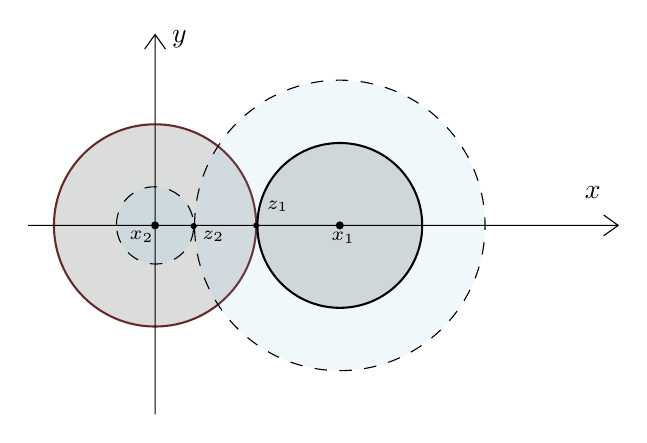
\begin{tikzpicture}[x=0.75pt,y=0.75pt,yscale=-1,xscale=1]
%uncomment if require: \path (0,300); %set diagram left start at 0, and has height of 300

%Shape: Circle [id:dp8664458953041292] 
\draw  [color={rgb, 255:red, 105; green, 40; blue, 40 }  ,draw opacity=1 ][fill={rgb, 255:red, 3; green, 14; blue, 10 }  ,fill opacity=0.14 ][line width=0.75]  (162.28,113) .. controls (162.28,86.09) and (184.09,64.28) .. (211,64.28) .. controls (237.91,64.28) and (259.72,86.09) .. (259.72,113) .. controls (259.72,139.91) and (237.91,161.72) .. (211,161.72) .. controls (184.09,161.72) and (162.28,139.91) .. (162.28,113) -- cycle ;
%Shape: Circle [id:dp9773613984359779] 
\draw  [fill={rgb, 255:red, 127; green, 192; blue, 231 }  ,fill opacity=0.11 ][dash pattern={on 4.5pt off 4.5pt}] (230.03,113) .. controls (230.03,74.35) and (261.35,43.02) .. (300,43.02) .. controls (338.65,43.02) and (369.98,74.35) .. (369.98,113) .. controls (369.98,151.65) and (338.65,182.97) .. (300,182.97) .. controls (261.35,182.97) and (230.03,151.65) .. (230.03,113) -- cycle ;
%Shape: Circle [id:dp69609627994047] 
\draw  [fill={rgb, 255:red, 127; green, 192; blue, 231 }  ,fill opacity=0.14 ][dash pattern={on 4.5pt off 4.5pt}] (192.39,112.68) .. controls (192.39,102.39) and (200.72,94.21) .. (211,94.39) .. controls (221.28,94.56) and (229.61,103.04) .. (229.61,113.32) .. controls (229.61,123.61) and (221.28,131.79) .. (211,131.61) .. controls (200.72,131.44) and (192.39,122.96) .. (192.39,112.68) -- cycle ;
%Shape: Circle [id:dp6366499429105177] 
\draw  [color={rgb, 255:red, 0; green, 0; blue, 0 }  ,draw opacity=1 ][fill={rgb, 255:red, 3; green, 14; blue, 10 }  ,fill opacity=0.14 ][line width=0.75]  (260.29,113) .. controls (260.29,91.07) and (278.07,73.29) .. (300,73.29) .. controls (321.93,73.29) and (339.71,91.07) .. (339.71,113) .. controls (339.71,134.93) and (321.93,152.71) .. (300,152.71) .. controls (278.07,152.71) and (260.29,134.93) .. (260.29,113) -- cycle ;
%Shape: Axis 2D [id:dp40333334108998553] 
\draw  (149.89,113) -- (434.13,113)(211,21) -- (211,204) (427.13,108) -- (434.13,113) -- (427.13,118) (206,28) -- (211,21) -- (216,28)  ;
%Shape: Ellipse [id:dp5618777383770377] 
\draw  [fill={rgb, 255:red, 0; green, 0; blue, 0 }  ,fill opacity=1 ] (209.35,113) .. controls (209.35,112.08) and (210.09,111.34) .. (211,111.34) .. controls (211.91,111.34) and (212.65,112.08) .. (212.65,113) .. controls (212.65,113.92) and (211.91,114.66) .. (211,114.66) .. controls (210.09,114.66) and (209.35,113.92) .. (209.35,113) -- cycle ;
%Shape: Ellipse [id:dp1723534686260293] 
\draw  [fill={rgb, 255:red, 0; green, 0; blue, 0 }  ,fill opacity=1 ] (298.35,113) .. controls (298.35,112.08) and (299.09,111.34) .. (300,111.34) .. controls (300.91,111.34) and (301.65,112.08) .. (301.65,113) .. controls (301.65,113.92) and (300.91,114.66) .. (300,114.66) .. controls (299.09,114.66) and (298.35,113.92) .. (298.35,113) -- cycle ;
%Shape: Circle [id:dp823378702207272] 
\draw  [fill={rgb, 255:red, 0; green, 0; blue, 0 }  ,fill opacity=1 ] (258.56,113) .. controls (258.56,112.36) and (259.08,111.84) .. (259.72,111.84) .. controls (260.36,111.84) and (260.87,112.36) .. (260.87,113) .. controls (260.87,113.64) and (260.36,114.16) .. (259.72,114.16) .. controls (259.08,114.16) and (258.56,113.64) .. (258.56,113) -- cycle ;
%Shape: Circle [id:dp9184097105556417] 
\draw  [fill={rgb, 255:red, 0; green, 0; blue, 0 }  ,fill opacity=1 ] (228.41,113.32) .. controls (228.41,112.66) and (228.95,112.12) .. (229.61,112.12) .. controls (230.27,112.12) and (230.81,112.66) .. (230.81,113.32) .. controls (230.81,113.99) and (230.27,114.52) .. (229.61,114.52) .. controls (228.95,114.52) and (228.41,113.99) .. (228.41,113.32) -- cycle ;

% Text Node
\draw (416.8,92.8) node [anchor=north west][inner sep=0.75pt]   [align=left] {$\displaystyle x$};
% Text Node
\draw (218,18) node [anchor=north west][inner sep=0.75pt]   [align=left] {$\displaystyle y$};
% Text Node
\draw (263.67,99.83) node [anchor=north west][inner sep=0.75pt]  [font=\scriptsize] [align=left] {$\displaystyle z_{1}$};
% Text Node
\draw (232.68,114.3) node [anchor=north west][inner sep=0.75pt]  [font=\scriptsize] [align=left] {$\displaystyle z_{2}$};
% Text Node
\draw (294.8,115) node [anchor=north west][inner sep=0.75pt]  [font=\scriptsize] [align=left] {$\displaystyle x_{1}$};
% Text Node
\draw (197.65,114.7) node [anchor=north west][inner sep=0.75pt]  [font=\scriptsize] [align=left] {$\displaystyle x_{2}$};


\end{tikzpicture}
    } 
        \caption{Последствия неточной оценки константы липшица. Пересечение серых кругов $z_1$ -- точное решение. Однако алгоритм находит $z_2$ из-за неправильной оценки констант.}
\end{center}
\label{fig:theorem_example}
\end{figure}

\end{comments}

